\chapter[Cadre théorique]{Cadre théorique (terminologie et concepts fondamentaux) \label{ch:sci_framework}}

\section{Introduction} % quoi que comment le contexte
% "le cadre théorique et définition des concepts de base de notre travail."
Ce chapitre est dédié à la présentation et l'explication des théories, termes et concepts nécessaires à la compréhension du présent mémoire.
Cependant, il ne s'agit pas d'explications approfondies mais d'une première approche % TODO faire une explication claire
L'objectif n'est pas de fournir des explications approfondies, mais plus de fournir les connaissances minimales à la compréhension du contenu et des enjeux du rapport.

De nombreux extraits provenant de Wikipédia seront utilisés dans cette partie. L'intérêt desdits extraits n'est pas leur exactitude scientifique, mais leur capacité à cerner le sens global des termes en quelques phrases simples.
D'autres sources plus fiables seront utilisées en complément, afin d'affiner les explications. 

Dans un premier temps, les domaines scientifiques dans lequel s'inscrit le stage seront brièvement définis.
Dans un second temps, les concepts et termes fondamentaux utilisés dans ce mémoire seront expliqués.
Enfin, pour situer le stage dans son contexte scientifique actuel, un aperçu de l'état de l'art dans la littérature sera donné.

\section{Doimaines scientifiques et techniques concernés} % définitions du domaine global
Ce stage s'inscrit dans deux principaux domaines :
\begin{itemize}
	\item l'\gls{dl}, une des branches de l'\gls{ml};
	\item le \glsfirst{nlp}.
\end{itemize}

\subsection{\Glsentrytext{ml}} \label{subsec:ml}\label{def:ml}
L'\glsfirst{ml} est un ensemble de \og méthodes [statistiques] permettant à une machine (au sens large) d'évoluer par un processus systématique, et ainsi de remplir des tâches difficiles ou problématiques par des moyens algorithmiques plus classiques\fg{}. D'après Wikipédia \footfullcite{wiki_ml}.

\subsection{\Glsentrytext{dl}} \label{subsec:dl}\label{def:dl}
L'\gls{dl} représente un ensemble de techniques de \gls{ml}, basés sur les techniques appelées \glspl{nn}.

Faisant partie des méthodes du \gls{ml}, l'\gls{dl} regroupe à la fois les méthodes de création, d'entraînement, d'optimisation et d'utilisation des modèles basés sur des \glspl{nn}.

\subsection{\Glsentrytext{nlp}} \label{subsec:nlp}\label{def:nlp}
Le \glsfirst{nlp} est une discipline qui s'intéresse au traitement des informations langagières par des moyens formels ou informatiques.

\section{Concepts et termes fondamentaux} % définition spécifique
\subsection{Définitions générales}
\begin{description}
	\item[\Gls{nn}\label{def:nn}]
	Un réseau de neurones artificiels ou réseau de neurones (\foreign{Neural Network} en anglais) est un \og ensemble de neurones formels interconnectés permettant la résolution de problèmes complexes tels que la reconnaissance des formes ou le traitement du langage naturel, grâce à l'ajustement des coefficients de pondération dans une phase d'apprentissage.\fg{} D'après Futura\footfullcite{futura_nn}.
	
	%%%%%
	%TODO 
\end{description}

\subsection{Concepts récurrents en \Glsentrytext{ml}}
\subsubsection{\Glsentrytext{model}\label{def:model}}
Un \gls{model} en \gls{ml} est la représentation du monde construite lors de l'apprentissage afin de répondre au problème à résoudre.

Dans le cadre de l'\gls{dl}, un modèle correspond généralement au réseau de neurone.

\subsubsection{Entraînement du modèle}
L'entraînement du \gls{model}, aussi appelé apprentissage, est le processus par lequel on adapte le \gls{model} de façon à mieux résoudre le problème.

\subsubsection{Données d'entraînement}\label{def:preprocessing}
Pour entraîner un \gls{model}, il faut lui fournir des données.
Généralement, on effectue un \gls{preprocessing}. Cela peut être retirer les données erronées, en adapter le format, les anonymiser, ou associer le résultat attendu aux données correspondants.

\subsection{\Glsentrytext{lm}}
\subsection{Principe des réseaux de neurones artificiels}
%http://www.statsoft.fr/concepts-statistiques/reseaux-de-neurones-automatises/reseaux-de-neurones-automatises.htm#type
\autocite{statsoft-nn}
Nous allons voir maintenant les principes de base des \glspl{nn}, sans nous attarder sur les principes mathématiques et statistiques sous-jacents.

\subsubsection{Le neurone formel}
Un neurone formel un objet mathématique qui synthétise des informations puis qui les transforme\autocite{datamining-nn}. C'est la brique fondamentale du réseau de neurone.

Il est essentiellement caractérisé par~:
\begin{itemize}
	\item \textbf{des entrées}~: la source des informations à synthétiser~;
	\item \textbf{une fonction de combinaison}~: la fonction dirigeant la synthèse des informations~;
	\item \textbf{une fonction d'activation}~: la fonction de transformation des informations synthétisées.
\end{itemize}

\begin{figure}[h]
	\centering
	%\rotatebox{90}{\scalebox{0.9}{\usetikzlibrary{arrows,shapes,positioning,shadows,trees}

\tikzset{
  basic/.style  = {draw, rounded corners=2pt, thin, text width=10em, drop shadow, rectangle},
  root/.style   = {basic, align=center,
                   fill=blue!30},
  level 1/.style={sibling distance=12em, level distance=5em},
  level 2/.style = {basic, align=center, fill=green!30},
  level 3/.style = {basic, rounded corners=2pt, thin, align=left, fill=pink!60, text width=16em, yshift=-2em}
}

\begin{tikzpicture}[
  edge from parent path={[->](\tikzparentnode.south) -- ++(0,-0.5em)
			-| (\tikzchildnode.north)},
  >=latex]

% root of the the initial tree, level 1
\node[root](loria) {LORIA}
% The first level, as children of the initial tree
  child {node[level 2] (c1) {D\'{e}partement 1:\\Algorithmique, calcul, image et g\'{e}om\'{e}trie}}
  child {node[level 2] (c2) {D\'{e}partement 2:\\M\'{e}thodes formelles}}
  child {node[level 2] (c3) {D\'{e}partement 3:\\R\'{e}seaux, syst\`{e}mes et services}}
  child {node[level 2, fill=green!60!] (c4) {D\'{e}partement 4:\\Traitement automatique des langues et des connaissances}}
  child {node[level 2] (c5) {D\'{e}partement 5:\\Syst\`{e}mes complexes, intelligence artificielle et robotique}};

% The second level, relatively positioned nodes
\begin{scope}[every node/.style={level 3}]
% \node [below of = c1, xshift=1em] (c11) {Setting shape};
% \node [below of = c11] (c12) {Choosing color};
% \node [below of = c12] (c13) {Adding shading};
\node [below of = c4, xshift=5em, yshift=-0.75em] (c41) {CELLO:\\\textit{Computational Epistemic Logic in LOrraine}};
\node [below of = c41] (c42) {MULTISPEECH:\\Analyse, perception et reconnaissance automatique de la parole};
\node [below of = c42] (c43) {ORPAILLEUR:\\Extraction et représentation de connaissances};
\node [below of = c43] (c44) {READ:\\Reconnaissance de l’écriture \& analyse de documents};
\node [below of = c44] (c45) {SMarT:\\\textit{Statistical Machine Translation \& Speech Modelization and Text}};
\node [below of = c45, yshift=0.5em] (c46) {SEMAGRAMME:\\Linguistique computationnelle};
\node [below of = c46, fill=red!40] (c47) {SYNALP:\\Traitement automatique des langues naturelles par méthode statistique et symbolique};
\end{scope}

% lines from each level 1 node to every one of its "children"
% \foreach \value in {1,...,5}
%   \draw[->] (loria.south) -| (c\value.north);
\foreach \value in {1,...,7}
  \draw[->] (c4.208) |- (c4\value.west);
\end{tikzpicture}}}
	\scalebox{1}{\def\layersep{3cm}
\begin{tikzpicture}[shorten >=1pt,->,draw=black!50, node distance=\layersep]
    \tikzstyle{every pin edge}=[<-,shorten <=1pt]
    \tikzstyle{input}=[rectangle];
    \tikzstyle{output neuron}=[circle,minimum size=20pt, fill=red!50];
    \tikzstyle{nonlinearity}=[rectangle,minimum size=20pt, fill=blue!50];
    \tikzstyle{annot} = [text width=6em, text centered]

    % Draw the input layer nodes
    \foreach \name / \y in {1,...,4}
    % This is the same as writing \foreach \name / \y in {1/1,2/2,3/3,4/4}
        \node[input] (I-\name) at (0,-\y) {Entr\'{e}e \y};

    % Draw the output layer node
    \node[output neuron, right of=I-1,xshift=-.5cm] (Syn) at (,-2.5) {};
    % Draw the output layer node
    \node[nonlinearity,pin={[pin edge={->}]right:Sortie}, right of=Syn] (NL) {};

    % Connect every node in the input layer with every node in the
    % hidden layer.
    \foreach \source in {1,...,4}
        \path (I-\source.east) edge (Syn);
	\path (Syn) edge (NL);

    % Annotate the layers
    \node[annot,above of=I-1, node distance=1.5cm] (hl) {Entr\'{e}es};
    \node[annot,above of=Syn] (hl) {Fonction de combinaison};
    \node[annot,above of=NL] (hl) {Fonction d'activation};
\end{tikzpicture}}
	\caption{Neurone formel basique}
	\label{fig:formal_neuron}
\end{figure}

\paragraph{Généralement en \gls{dl}:}
\begin{itemize}
	\item les neurones formels manipulent des nombres~;
	\item la neurones fonction de combinaison est une somme pondérée des entrées, alors \textbf{caractérisée par les poids} attribués à chaque entrée~; \label{def:weight1}
	\item la fonction d'activation est généralement une fonction non linéaire (comme $\tanh$), alors appelée \textbf{\gls{nonlinearite}}~; \label{def:nonlinearite}
	\item les entrées sont soit les sorties d'autres neurones, sont soit les entrées du réseau. Cela nous mène à la partie suivante.
\end{itemize}

\begin{figure}[h]
	\centering
	\scalebox{1}{\newsavebox\myboxa
\savebox\myboxa{%
	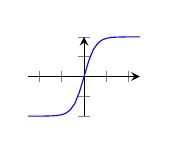
\begin{tikzpicture}
		\begin{axis}[
		  axis lines=middle,
		  width=3cm,
		  xticklabels={,,},
		  yticklabels={,,}
		]
		\addplot+[no marks] {tanh(x)};
		\end{axis}
	\end{tikzpicture}%
}

\def\layersep{3cm}
\begin{tikzpicture}[shorten >=1pt,->,draw=black!50, node distance=\layersep]
    \tikzstyle{every pin edge}=[<-,shorten <=1pt]
    \tikzstyle{input}=[rectangle];
    \tikzstyle{weight}=[circle,minimum size=20pt, fill=green!50,xshift=-1cm];
    \tikzstyle{output neuron}=[circle,minimum size=20pt, fill=red!50];
    \tikzstyle{nonlinearity}=[rectangle,minimum size=20pt, fill=blue!30];
    \tikzstyle{annot} = [text width=6em, text centered]

    % Draw the input layer nodes
    \foreach \name / \y in {1,...,4}
    % This is the same as writing \foreach \name / \y in {1/1,2/2,3/3,4/4}
        \node[input] (I-\name) at (0,-\y) {Entr\'{e}e \y};
    \foreach \name / \y in {1,...,4}
        \node[weight,right of=(I-\name)] (W-\name) at (1,-\y) {$P\name$};

    % Draw the output layer node
    \node[output neuron, right of=I-1, right of=I-2,xshift=-1cm] (Syn) at (,-2.5) {$\Sigma$};
    % Draw the output layer node
    \node[nonlinearity,pin={[pin edge={->}]right:Sortie}, right of=Syn,label=above:$\tanh$] (NL) {\usebox\myboxa};

    % Connect every node in the input layer with every node in the
    % hidden layer.
    \foreach \source in {1,...,4}
        \path (I-\source.east) edge (W-\source.west);
    \foreach \source in {1,...,4}
        \path (W-\source.east) edge (Syn);
	\path (Syn) edge (NL);

    % Annotate the layers
    \node[annot,above of=I-1, node distance=1.5cm] (hl) {Entr\'{e}es};
    \node[annot,above of=W-1, node distance=1.5cm] (pl) {Poids};
    \node[annot,above of=Syn] (sl) {Somme};
    \node[annot,above of=pl, above of=sl, node distance=.5cm,text width=12em,xshift=-1.5cm] (hl) {Somme pond\'{e}r\'{e}e};
    \node[annot,above of=NL] (hl) {Non-lin\'{e}arit\'{e}};
\end{tikzpicture}}
	\caption[Exemple de neurone formel en \glsentrytext{dl}]{Exemple de neurone formel en \gls{dl}, avec une $tanh$ pour \gls{nonlinearite}.}
	\label{fig:formal_neuron_dl}
\end{figure}

\subsubsection{Les réseaux et les couches\label{subsec:network}}
Les \glspl{nn} sont des réseaux composés de neurones formels, dont les sorties des uns servent d'entrées aux autres.

Il en existe de nombreuses architectures, mais toutes celles dont nous parlerons dans ce rapport sont organisées en couches.
En \gls{dl}, on parle de couches cachées pour toutes les couches situées entre la couche d'entrée et celle de sortie du réseau. La \autoref{fig:nn} représente un \gls{nn} en trois couches.

\begin{figure}[h]
	\centering
	\scalebox{1}{\def\layersep{2.5cm}
\begin{tikzpicture}[shorten >=1pt,->,draw=black!50, node distance=\layersep]
    \tikzstyle{every pin edge}=[<-,shorten <=1pt]
    \tikzstyle{neuron}=[circle,fill=black!25,minimum size=17pt,inner sep=0pt]
    \tikzstyle{input neuron}=[neuron, fill=green!50];
    \tikzstyle{output neuron}=[neuron, fill=red!50];
    \tikzstyle{hidden neuron}=[neuron, fill=blue!50];
    \tikzstyle{annot} = [text width=4em, text centered]

    % Draw the input layer nodes
    \foreach \name / \y in {1,...,4}
    % This is the same as writing \foreach \name / \y in {1/1,2/2,3/3,4/4}
        \node[input neuron, pin=left:Entr\'{e}e \y] (I-\name) at (0,-\y) {};

    % Draw the hidden layer nodes
    \foreach \name / \y in {1,...,5}
        \path[yshift=0.5cm]
            node[hidden neuron] (H-\name) at (\layersep,-\y cm) {};

    % Draw the output layer node
    \node[output neuron,pin={[pin edge={->}]right:Sortie}, right of=H-3] (O) {};

    % Connect every node in the input layer with every node in the
    % hidden layer.
    \foreach \source in {1,...,4}
        \foreach \dest in {1,...,5}
            \path (I-\source) edge (H-\dest);

    % Connect every node in the hidden layer with the output layer
    \foreach \source in {1,...,5}
        \path (H-\source) edge (O);

    % Annotate the layers
    \node[annot,above of=H-1, node distance=1cm] (hl) {Couche cach\'{e}e};
    \node[annot,left of=hl] {Couche d'entr\'{e}e};
    \node[annot,right of=hl] {Couche de sortie};
\end{tikzpicture}}
	\caption[Réseau de neurones en 3 couches]{Réseau de neurones en 3 couches, de respectivement 4, 5 et 1 neurones. Les couches sont complètement connectées entre elles.}
	\label{fig:nn}
\end{figure}

\subsubsection{L'entraînement des réseaux de neurones}
Une des façons d'entraîner un \gls{nn} est de lui présenter des données, et de comparer les résultats produits par le \gls{nn} avec les résultats attendus.

On cherche ensuite à minimiser l'écart entre résultats produits et attendus.
La technique de la \og rétro-propagation du gradient\fg{} permet de connaître l'implication de chacun des paramètres du modèle dans l'écart des résultats, et de les mettre à jour de façon à minimiser l'écart.
Cette technique est mise en œuvre informatiquement par la \gls{automatic differentiation}. % TODO nécessaire ou pas du tout ?

\subsubsection{La représentation sous forme matricielle}
\label{def:weight2}
Il existe une représentation des \glspl{nn} sous forme de matrice.

Cette représentation 

Pour expliquer cette représentation, nous allons
 --->> Exemple


-> GPU
\subsubsection{Les assemblages de modules et la programmation différentielle}
\autoref{diff_prog}


\subsection{Les types de réseaux de neurones artificiels}
\subsubsection{Les Réseaux \foreign{feedforward}}
\subsubsection{Les Réseaux de Neurones Artificiels Récurrents} \label{def:rnn}
Un Réseau de Neurones Artificiels Récurrents, plus simplement \gls{rnn} en anglais) est un réseau de neurones artificiels suivant une architecture dite récurrente.

Ce genre de réseau est utilisé pour travailler avec des séquences d'entrées 
et/ou de sorties; il y a transmission d'information entre chaque élément de 
la séquence. \footfullcite{wiki_rnn}%TODO describe RNN

%TODO schema explicattif
%TODO cas particulier du LSTM et du GRU

Il existe de nombreuses variantes d'architectures récurrentes pour les \gls{nn}, en plus de l'architecture de base que nous venons de présenter.
En voici deux, dont nous reparlerons plus loin dans le rapport:
\begin{description}
	\item[\Gls{gru}\label{def:gru}]
	%%%%%
	\item[\Gls{lstm}\label{def:lstm}]
\end{description}
\subsubsection{Quelques autres types non détaillés}
CNN


\section{État de l'art\label{sec:soa}}
\subsection{\Glsentrytext{project_gmsnn}}
\subsection{\Glsentrytext{project_papud}}

--> next parts
